\documentclass[12pt]{report}
\usepackage[top=1in, bottom=1in, left=1in, right=1in, a4paper]{geometry}

 \ifx\pdftexversion\undefined
 \usepackage[dvips]{graphicx}
 \else
 
 \usepackage[pdftex]{graphicx}
 \DeclareGraphicsRule{*}{mps}{*}{}
 \fi
%\usepackage{tabularx,colortbl}
\usepackage{url}
\usepackage{chapterbib}
\usepackage{hyperref}
\usepackage{tabularx}
%\usepackage{tikz}
%\usepackage{pgfplots}
%\usepgfplotslibrary{groupplots} 
%\usepackage{pgf, pgfarrows, pgfnodes}
\usepackage{lscape}
\usepackage{longtable}
\usepackage{float}
\usepackage{url}
\usepackage{multicol}
\usepackage{color}
\usepackage{float}

%\usepackage[none]{hyphenat}
\renewcommand{\bibname}{References}

\setcounter{secnumdepth}{4}
\setcounter{tocdepth}{4}

\begin{document}

\begin{titlepage}
 \begin{center}
\LARGE
\textbf{Cloud based IT Infra with Central Identity} \\
\vfill
\large
\textbf{\{ Project reboot \}}\\
\vfill
\textbf{Phase - I Project Report }\\
\vfill
\Large
\underline{\textbf{Project Guide }} \\ 
\large
\underline{} \\
T. Chandra Shaker \\
\small
Dept. of CSE -- RGUKT Nuzvid \\
\small
\url{chandra.indra@gmail.com}
\vfill

\Large
\textbf{\underline{ Project Team } } \\
\underline{} \\
\large
\begin{tabular}{l  l}
T. Aneesh Kumar & N090247  \\
P. Nageswarao  & N091030  \\
P. Anesh  & N090977  \\
P. Jyothi Ram & N090990  \\
K. Naresh Chowdary  & N090331  \\
N. Venkata Sateesh  & N090935  \\
M. Sanyasi Rao & N090891 
\end{tabular}

\vfill



\includegraphics[width=3.5cm]{rgukt_logo.jpg} 
\Large
\underline{} \\
\underline{} \\
\normalsize
\textbf{Dept. of Computer Science and Engg. } \\
\textbf{R.G.U.K.T. - Nuzvid } \\
\textbf{Krishna Dt. - Andrha Pradesh - 521202}


\normalsize
\vfill
%\begin{multicols}{2}
%\begin{flushleft}
%\textbf{Start Date} : Sep 2014 \\
%\end{flushleft}
%
%
%\begin{flushright}
%\textbf{End Date} : Jan 2015 \\
%\end{flushright}
%\end{multicols}

\textbf{Sep 2014 -- Dec 2014 }

\end{center}
\end{titlepage}

% \pagebreak \thispagestyle{empty} \textcolor{white}{text} \pagebreak
 
\chapter*{Abstract}
\setcounter{page}{1}
\pagenumbering{roman}
\normalsize
\hspace{0.5cm} The main objective of ``Cloud based IT Infra with Central Identity'' is to utilize exisiting hardware, turn them into private clouds and access all of its services using 
Central Identity, which can be available to third party developers as API with dynamic role management and service endpoints. \newline

New private cloud based IT Infra is aimed to develop using some opensource tools like OpenStack, NFS, LDAP, Ubuntu and etc \newline

Expecting to surve with high computational virtual machines to the research, academic, learning purpose, virtal labs rather than dedicated lab hardware.

%\pagebreak \thispagestyle{empty} \textcolor{white}{text} \pagebreak

\setcounter{page}{2}
\pagenumbering{roman}
\tableofcontents
\listoffigures
\listoftables
\pagebreak \thispagestyle{empty} \pagebreak

 
\setcounter{page}{1}
\pagenumbering{arabic}


\chapter{Introduction}

\section{Introduction}
	``Cloud Based IT Infra with Central Identity'' is a complete solution, based on private cloud to enhance and effiecient utilization the IT Infrastructure of an emerging Universities and Organizations with Central Identity for all its users to access its services.\newline

	It is going to be developed in 3 phases 
	\begin{itemize}
		\item \textit{Private cloud} 
		\item \textit{Deploying Network Services} 
		\item \textit{Central Identity}
	\end{itemize}
	
\subsection{Private Cloud}

	Private Cloud establishment is targeted for hardware resource pooling, providing high computational and scalable virtual machines for deploying network based applications (smtp, proxy, ftp), web application and Network storage.
	
\subsection{Deploying Network Services}

	Configuration of Uniform hardware experience over the complete university includes single sign on on every device, configuration of mail servers etc.
	
\subsection{Central Identity}

	Essential part that combines normal network services(proxy, mail, etc.) and organizational web \& native applications. In addtion to that this central identity is available to thrid party developers as API with dynamic based role user authentication protocols.	
	

\chapter{Motivation \& Approach}

\section{Existing System}

%	We have been observing that components we are planed develop name private cloud and central identity are already exsisted but key difference here is we want to combine them and extend the central identity as Identity as a service to all emerging developers in that organization with some sort of API calls in  

\begin{itemize}
	\item The environment we observed is our university, it cosists of 7000 students and more than 500+ faculty with 6 core Engg. departments apart from 2 years of PUC course.
	\item Each Department is having strength of 700 students they arrenged these students into various various classes of 60 to 70 each, total 10 to 12 number. 
	\item Each student is provided with one Laptop with 2G RAM, 1.5GHz Clock speed and 200 GB Harddisk Storage. 
	\item All students are using these sytems for more than 8 hours in a day.
	\item All these students has to provided with course content and course labs, they are maitaining dedicated labs with 50 - 60 machines.
	
\end{itemize}


\section{Problems under consideration}

	We have observed these problems over our University
	
	\begin{itemize}
		\item Failed to maintain large user load web services  and network applications.
		\item No Central Identity, Storage \& High capacity hardware resource pool.
		%\item Redundent data in each prospect
		\item Inadequate resource requirements for Research.
		\item Dedicated computer course labs like Matlab, VLSI, etc. and these labs are useful only at lab hourse most of time they are idle.
		\item Redendent data and failed to moniter the content over student laptops.
	\end{itemize}

\section{Proposed System}

	To avoid above mentioned observations we are proposing one new system with 
	\begin{itemize}
		\item Cloud based hardware resources clustering.
		\item Central Identity for Network Applicaitons with REST API.
		\item Dynamic user role management.
		\item Providing Virtual Labs (MatLab, etc.,).
		\item High Configurational Virtual Machines for research.
	\end{itemize}
	
\section{Approach}

	We want to make use of entire departmental hardaware resources more on its students laptops capacity and create a common pool of resources hence easy to maintain and moniter.\\
	
	We want to provide signle sign on implentation in each class of 60-70 laptops. such that user can use his own unique username to access university resources and later he can use the same password for network based or web based applications such as updates, mails, examinations, results etc.\newline
	
	User data can be data is retrevied from the Storage server like nfs while loging in to his laptop in any class room and his laptop's computational and storage capacity is used by the private cloud extentions that it make his laptop as slave node when ever laptop is available.\newline 
	
	User can develop application and they can use Central Identity in their application with user control and access specifations for API calls.

%\chapter{System Design & Components}
%
%\section{System Design }
%\begin{figure}[H]
% \centering
% 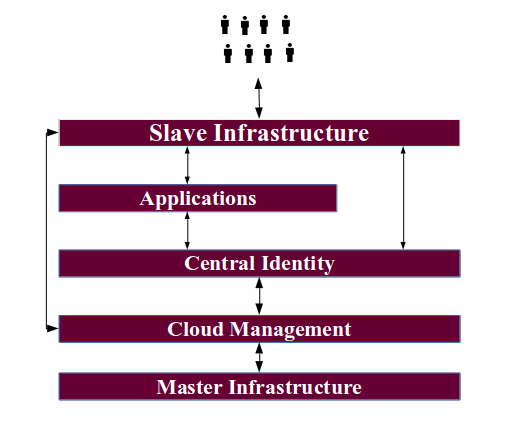
\includegraphics[width=8cm]{./idea.png}
% \caption{Developemnt Stack\label{fig:Developemnt Stack}}
%\end{figure}
%
%\section{Development Architecture}
%\begin{figure}[H]
% \centering
% 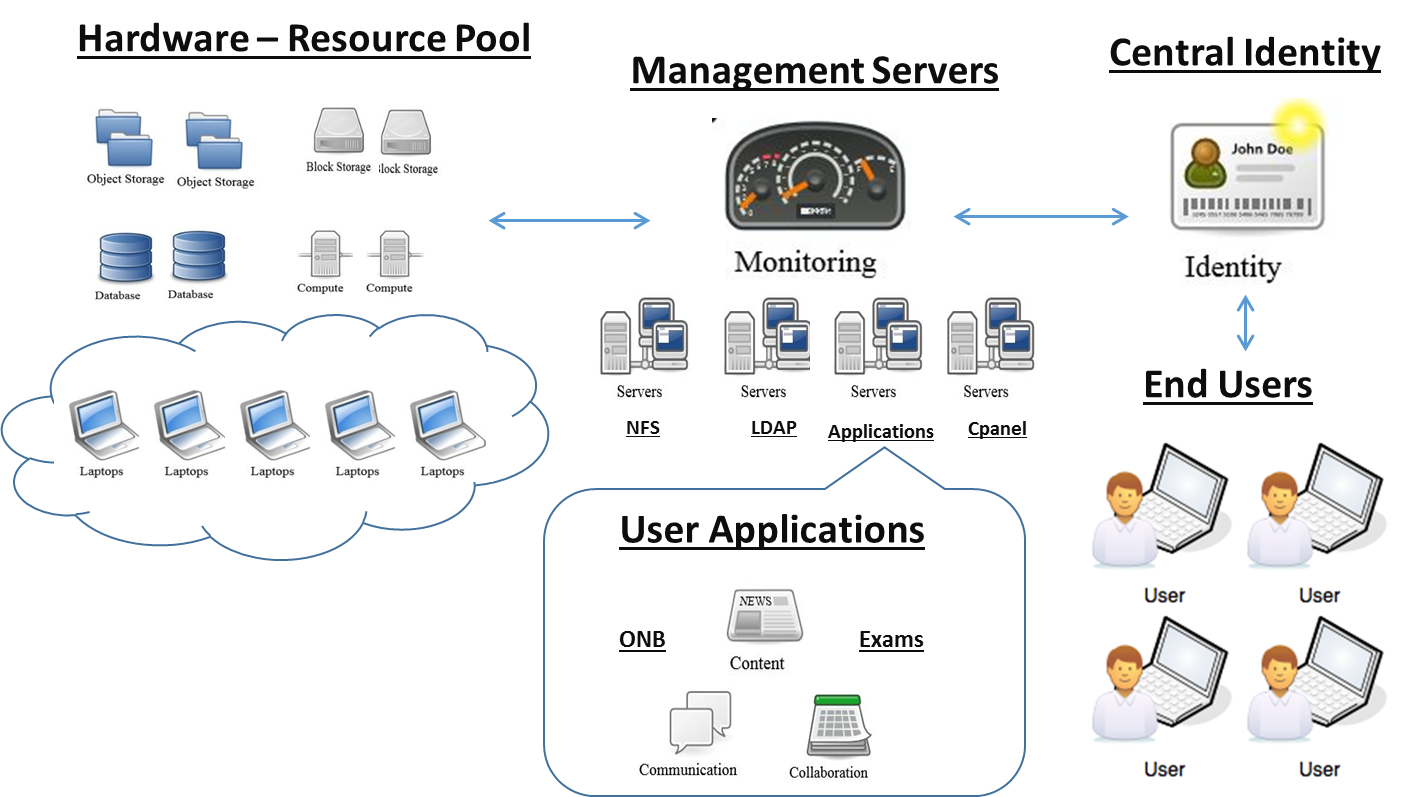
\includegraphics[width=10cm]{./all.png}
% \caption{Archtitecture\label{fig:Archtitecture}}
%\end{figure}

\chapter{Design View}
	
\section{Users \& IT Services}

	We are grouping all IT Services that are required for University into one and identifing the user who will going to use them. All Users are catagorized into 4 groups $ ^{[1]}$
	
	\begin{itemize}
	\item Studens
	\item Developers
	\item Staff, faculty
	\item Researches
	\end{itemize}
	
\begin{figure}[H]
\begin{center}
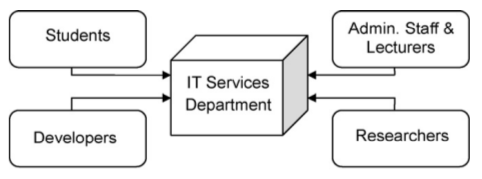
\includegraphics[width=7cm]{./it.png}
\caption{ Simplified structure of the main users of IT services in a typical university. \label{fig:Simplified structure of the main users of IT services in a typical university. }}
\end{center}
\end{figure}
	
	All University IT Services are deployed in a private cloud, constructed over exsiting infrastructure, that can be browdly viewed as 
	
\begin{figure}[H]
\begin{center}
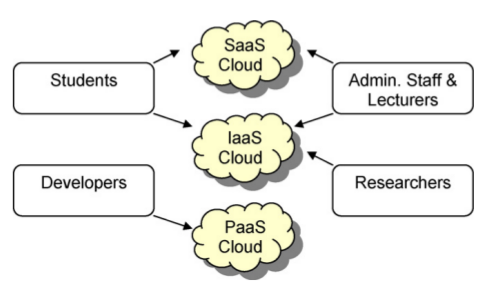
\includegraphics[width=7cm]{./it2.png}
\caption{ Simplified structure of the main users of IT services in a typical university now using the services of cloud computing\label{fig:Simplified structure of the main users of IT services in a typical university now using the services of cloud computing. }}
\end{center}
\end{figure}	
	
	
\section{Components Identified}

In this project we are restricting ourselves to some componets of the above mentioned system, we are planing to develop them in upcoming semister. We have done literature survey about these componets

\begin{itemize}
	\item Central Identiy 
	\begin{itemize}
		\item Single Sign on
		\item Fedarated Identity
		\item Dynamic Role Based Access Control
		\item REST API to third party
	\end{itemize}
	\item Network Components Configurations
	\begin{itemize}
		\item AAA, LDAP, NFS
	\end{itemize}
	\item Construction of private cloud
	\begin{itemize}
		\item Openstack, 
	\end{itemize}
\end{itemize}


	
\chapter{Implentation and Specifications}

\section{Implentation}

	For maintining above kind of envronment we have to setup one private cloud which will gives the highly scalable virtual machines to server the user need services on fly.\\
	
	We want develop minal system with the above guidelines in a lab environment of 10 Master nodes and 5 client machines with uniform operating system and nfs data share. Later extended upto departmental level.
	
	
\section{Specifications}

	\begin{itemize}
		\item 15 Laptops with below configuration ( 10 Master Nodes + 5 Slave Nodes )
			\begin{itemize}
				\item 4GB RAM, 500 GB Harddisk, Intel i3 processor 1.5GHz Clock
			\end{itemize}
		
		\item Class C Network 
			\begin{itemize}
			 	\item Static IP for Master Nodes
			 	\item DHCP / Static IP for Slave Nodes
			\end{itemize}
			
		\item Uninterrupted power suply for Master Nodes.
		
	\end{itemize}
	
\section{Desired Technologies}

	\begin{itemize}
		\item Opensource private cluod tools such as Openstack, Cloudstack, etc.
		\item Ubuntu 14.04 Server LTS.
		\item LDAP Active Directories, Kerbrose, Squid for Network proxy.
		\item OAuth 2.0 with extended dynamic roles managment.
		\item Nodejs for Implementation of OAuth 2.0 as REST API.
		\item Git for Version control. 
		\item Ascii doc / python shpenix \& Latex for Documentation.
	\end{itemize}
	
\section{Expcted Results}

	We are expecting the below results after successfull implemenation of ``Cloud Based IT Infra with Central Identity'' in lab enviroment with above mentioned specifications

	\begin{itemize}	
	\item Hardware resoucre clusters from Master Nodes
	 \begin{itemize}
	 	\item 40 GB RAM
		\item 5TB of Hard disk
		\item 15 GHz Clock Speed	
	 \end{itemize}
		
	\item Hardware resoucre clusters from Slave Node (available only at active period)
	 \begin{itemize}
	 	\item 20 GB RAM
		\item 2TB of Hard disk
		\item 7.5 GHz Clock Speed	
	 \end{itemize}
	 
	\item Well Documented Implementation of Central Identity for 
	 \begin{itemize}
	 	\item Single Sign on of Client Machines.
	 	\item Network applications proxy, mails.
	 	\item University Web Services and Departmental websites.
	 	\item Third party OAuth 2.0 Implemenation as API. 
	 \end{itemize}
	\item Dynamic user role management for both Web and Native applications as API.
	\item Central Cloud Storage Pool.
	\item High Computational Virtual Machines.
	\item Virtual Labs insted of Dedicated labs in Remote Desktop or in SSH protocol.
	\item Content or Data Monitering in a Organization.
	\item Get full recovery and achieve more than 99.99\% services up time.
	\item Extendable to several departments and Universities.
	
	\end{itemize}
	

\chapter{References}

\section{Web References}

\begin{itemize}
\item Ubnutu OS, http://www.ubuntu.com/
\item Openstack, https://openstack.org/
\item Linux Bible, http://tuxnetworks.blogspot.com
\item OAuth 2.0, http://oauth.net/
\item Node.js https://nodejs.org
\item Git, https://github.com
\item Ascii doc, http://asciidoc.org
\item Bootstrap, http://getbootstrap.com 
\item Stack Overflow http://stackoverflow.com/

\end{itemize}
		

\end{document}